\documentclass[12pt,a4paper]{article}

\usepackage[utf8]{inputenc}
\usepackage[T1]{fontenc}
\usepackage[brazil]{babel}

\usepackage[margin=2.5cm]{geometry}

\usepackage{graphicx}
\usepackage{float}
\usepackage{booktabs}
\usepackage{caption}

\usepackage{amsmath,amssymb}

\usepackage{tikz}
\usetikzlibrary{positioning,arrows.meta,shapes,shadows}

\usepackage{xcolor}
\usepackage{listings}

\usepackage{hyperref}
\hypersetup{hidelinks}

\usepackage{fancyhdr}
\usepackage{setspace}
\usepackage{tocloft}

\lstset{
basicstyle=\ttfamily\small,
keywordstyle=\color{blue!70!black}\bfseries,
commentstyle=\color{gray},
stringstyle=\color{green!50!black},
showstringspaces=false,
breaklines=true,
numbers=left,
numberstyle=\tiny\color{gray},
frame=single,
language=Python,
tabsize=2,
breakatwhitespace=true
}

\setstretch{1.5}
\setlength{\parindent}{1.27cm}

\pagestyle{fancy}
\fancyhf{}
\fancyhead[R]{\small\textit{Análise de Colaboração em Repositórios GitHub}}
\fancyfoot[C]{\thepage}
\renewcommand{\headrulewidth}{0.4pt}

\begin{document}

%-------------------------------------------------
% CAPA
%-------------------------------------------------
\begin{titlepage}
\centering

\vspace*{2cm}

{\large PONTIFÍCIA UNIVERSIDADE CATÓLICA DE MINAS GERAIS\par}
{\large Curso de Engenharia de Software\par}

\vfill

{\Large\bfseries ANÁLISE DA REDE DE COLABORAÇÃO EM REPOSITÓRIOS DO GITHUB\par}

\vspace{0.5cm}

{\large Utilizando Teoria de Grafos\par}

\vfill

{\large
Davi Nunes Carvalho\\
Luiz Fernando Batista Moreira\\
Josué Carlos Goulart dos Reis\\
João Victor Russo Marquito
\par}

\vfill

{\large Belo Horizonte\par}
{\large Junho de 2026\par}

\end{titlepage}


%-------------------------------------------------
% RESUMO
%-------------------------------------------------
\begin{abstract}
Este trabalho apresenta uma ferramenta para análise de redes de colaboração em repositórios do GitHub utilizando Teoria de Grafos. O sistema modela interações entre colaboradores (comentários, revisões, merges e fechamentos de issues) como grafos ponderados direcionados. A implementação inclui duas representações de grafos (lista de adjacência e matriz de adjacência), integração com a API REST do GitHub, cálculo de 10+ métricas de análise de rede (PageRank, betweenness, closeness, eigenvector, clustering, assortatividade, detecção de comunidades e bridging ties) e exportação CSV compatível com o Gephi. O projeto foi validado com 84 testes unitários e executado sobre o repositório \texttt{devlikeapro/waha}.
\end{abstract}

\newpage

%-------------------------------------------------
% SUMÁRIO
%-------------------------------------------------
\thispagestyle{empty}
\tableofcontents
\newpage

\pagenumbering{arabic}
\setcounter{page}{1}



% ============================================================================
% 1. INTRODUÇÃO
% ============================================================================
\section{Introdução}\label{sec:intro}

Repositórios de software aberto no GitHub constituem redes sociotécnicas complexas onde colaboradores interagem através de múltiplos canais: comentários em \textit{issues}, discussões em \textit{pull requests}, revisões de código e decisões de integração. Essas interações formam uma estrutura subjacente que codifica padrões de influência, expertise e comunicação dentro do projeto.

A aplicação de Teoria de Grafos a essas redes permite quantificar e visualizar a dinâmica colaborativa. Representando usuários como vértices e interações como arestas ponderadas direcionadas, é possível identificar: (i) colaboradores centrais e influentes; (ii) estruturas de comunidades informais; (iii) usuários que atuam como conectores entre grupos isolados; (iv) padrões assortivos ou dissortativos de conexão. Essas informações são essenciais para compreender a governança e sustentabilidade de projetos open source.

\subsection{Objetivos}

\begin{enumerate}
  \item Implementar estruturas de dados de grafos em Python puro, sem bibliotecas especializadas, atendendo uma API completa com duas representações (\textit{adjacency list} e \textit{adjacency matrix})
  \item Modelar interações reais do GitHub como grafos ponderados direcionados, com acumulação automática de pesos em arestas paralelas
  \item Desenvolver um minerador robusto que coleta dados via API REST do GitHub, tratando autenticação, paginação e rate limits
  \item Implementar 10+ métricas de análise de redes complexas: centralidade de grau, betweenness, closeness, PageRank, eigenvector, clustering, assortatividade, densidade, detecção de comunidades e bridging ties
  \item Validar a ferramenta através de testes unitários e demonstrar exportação para Gephi
\end{enumerate}

% ============================================================================
% 2. MODELAGEM DO PROBLEMA
% ============================================================================
\section{Modelagem do Problema}\label{sec:modelagem}

\subsection{Justificativa da Escolha do Repositório}

O repositório \texttt{devlikeapro/waha} foi escolhido por possuir mais de 5.000 estrelas no GitHub, atendendo ao requisito de uma comunidade ativa e com grande volume de interações. O projeto WAHA (WhatsApp HTTP API) é uma solução open source que permite integrar aplicações ao WhatsApp por meio de APIs HTTP, sendo amplamente utilizada e mantida por diversos colaboradores.

Além da popularidade, o repositório apresenta uma quantidade significativa de issues, pull requests, revisões e comentários, fornecendo dados suficientes para modelar e analisar a rede de colaboração entre desenvolvedores. Essas características tornam o projeto adequado para a construção dos grafos de interação e para a aplicação das métricas de análise de redes propostas neste trabalho.

\subsection{Definição Formal}

O sistema constrói quatro grafos $G = (V, E)$ direcionados ponderados simples, onde:
\begin{align}
  V &= \{\text{logins únicos de usuários extraídos do repositório}\} \\
  E &\subseteq V \times V, \quad (u, v) \in E \Rightarrow u \neq v \text{ (sem self-loops)} \\
  w: E &\to \mathbb{R}^+ \quad \text{(peso acumulado de arestas)}
\end{align}

Os quatro grafos modelam diferentes dimensões de interação:
\begin{enumerate}
  \item \textbf{G1} — comentários em issues e pull requests (peso 2 por interação)
  \item \textbf{G2} — fechamentos de issues por outro usuário (peso não especificado no integrado)
  \item \textbf{G3} — revisões/aprovações e merges de pull requests (pesos 4 e 5)
  \item \textbf{Grafo Integrado} — fusão ponderada de G1, G2 e G3
\end{enumerate}

\subsection{Estratégia de Coleta de Dados}

O minerador \texttt{GithubMiner} segue: (i) autenticação via token em \texttt{.env}; (ii) paginação de issues (\texttt{per\_page=100}, 5 páginas); (iii) para cada item: coleta comentários, revisões, detalhes de merge; (iv) tratamento robusto de erros (ignora status $\neq$ 200).

\subsection{Transformação de Interações em Arestas}

Cada interação é convertida em aresta direcionada com acumulação de pesos:
\begin{itemize}
  \item \textbf{Comentário:} usuário $c$ comenta issue/PR aberta por $a \Rightarrow$ aresta $c \to a$ recebe $+2$ (G1 e integrado)
  \item \textbf{Abertura comentada:} se issue (não PR) recebe comentário de $c \neq a \Rightarrow$ aresta $a \to c$ recebe $+3$ (integrado; sinaliza envolvimento da comunidade)
  \item \textbf{Revisão/aprovação:} usuário $r$ revisa PR de $a \Rightarrow$ aresta $r \to a$ recebe $+4$ (G3 e integrado)
  \item \textbf{Merge:} usuário $m$ mergua PR de $a \Rightarrow$ aresta $m \to a$ recebe $+5$ (G3 e integrado)
  \item \textbf{Acumulação:} múltiplas interações do mesmo par $(u, v)$ somam seus pesos (e.g., 3 comentários = peso 6)
\end{itemize}

\subsection{Esquema de Pesos}

\begin{table}[h]
  \centering
  \caption{Pesos das interações no grafo integrado. Hierarquia reflete relevância para colaboração técnica.}
  \label{tab:pesos}
  \begin{tabular}{l|c|p{5.5cm}}
    \toprule
    \textbf{Interação} & \textbf{Peso} & \textbf{Semântica} \\
    \midrule
    Comentário em issue/PR & 2 & Participação leve (opinião, sugestão) \\
    Abertura comentada & 3 & Comunidade engajada na proposta \\
    Revisão/aprovação de PR & 4 & Análise técnica profunda \\
    Merge de PR & 5 & Decisão executiva de integração \\
    \bottomrule
  \end{tabular}
\end{table}

A hierarquia de pesos reflete a tese de que revisões e merges requerem expertise maior que comentários: um revisor avalia correção técnica; um merguer assume responsabilidade de integração. Comentários são participação essencial mas menos comprometida.

% ============================================================================
% 3. MODELAGEM DO SISTEMA
% ============================================================================
\section{Modelagem do Sistema}\label{sec:modelagem_sistema}

Esta seção apresenta os artefatos UML que descrevem a arquitetura estática, comportamental e os fluxos de execução da ferramenta.

% ----------------------------------------------------------------------------
\subsection{Diagrama de Classes}
% ----------------------------------------------------------------------------

O sistema organiza sua arquitetura em três principais responsabilidades. A classe abstrata \texttt{AbstractGraph} define uma interface comum para operações sobre grafos, sendo implementada pelas classes concretas \texttt{AdjacencyListGraph} e \texttt{AdjacencyMatrixGraph}. A primeira utiliza uma estrutura baseada em lista de adjacência \texttt{List[Dict[int, float]]}, sendo adequada para grafos esparsos, enquanto a segunda utiliza uma matriz de adjacência $N \times N$ com valores \texttt{float|None}, permitindo acesso direto às arestas. A classe \texttt{GithubMiner} é responsável pela coleta dos dados da API e pela construção das estruturas de grafo. Já a classe \texttt{GraphAnalytics} concentra os algoritmos de análise, incluindo métricas de centralidade, agrupamento e relacionamento entre os colaboradores.

\begin{figure}[H]
    \centering
    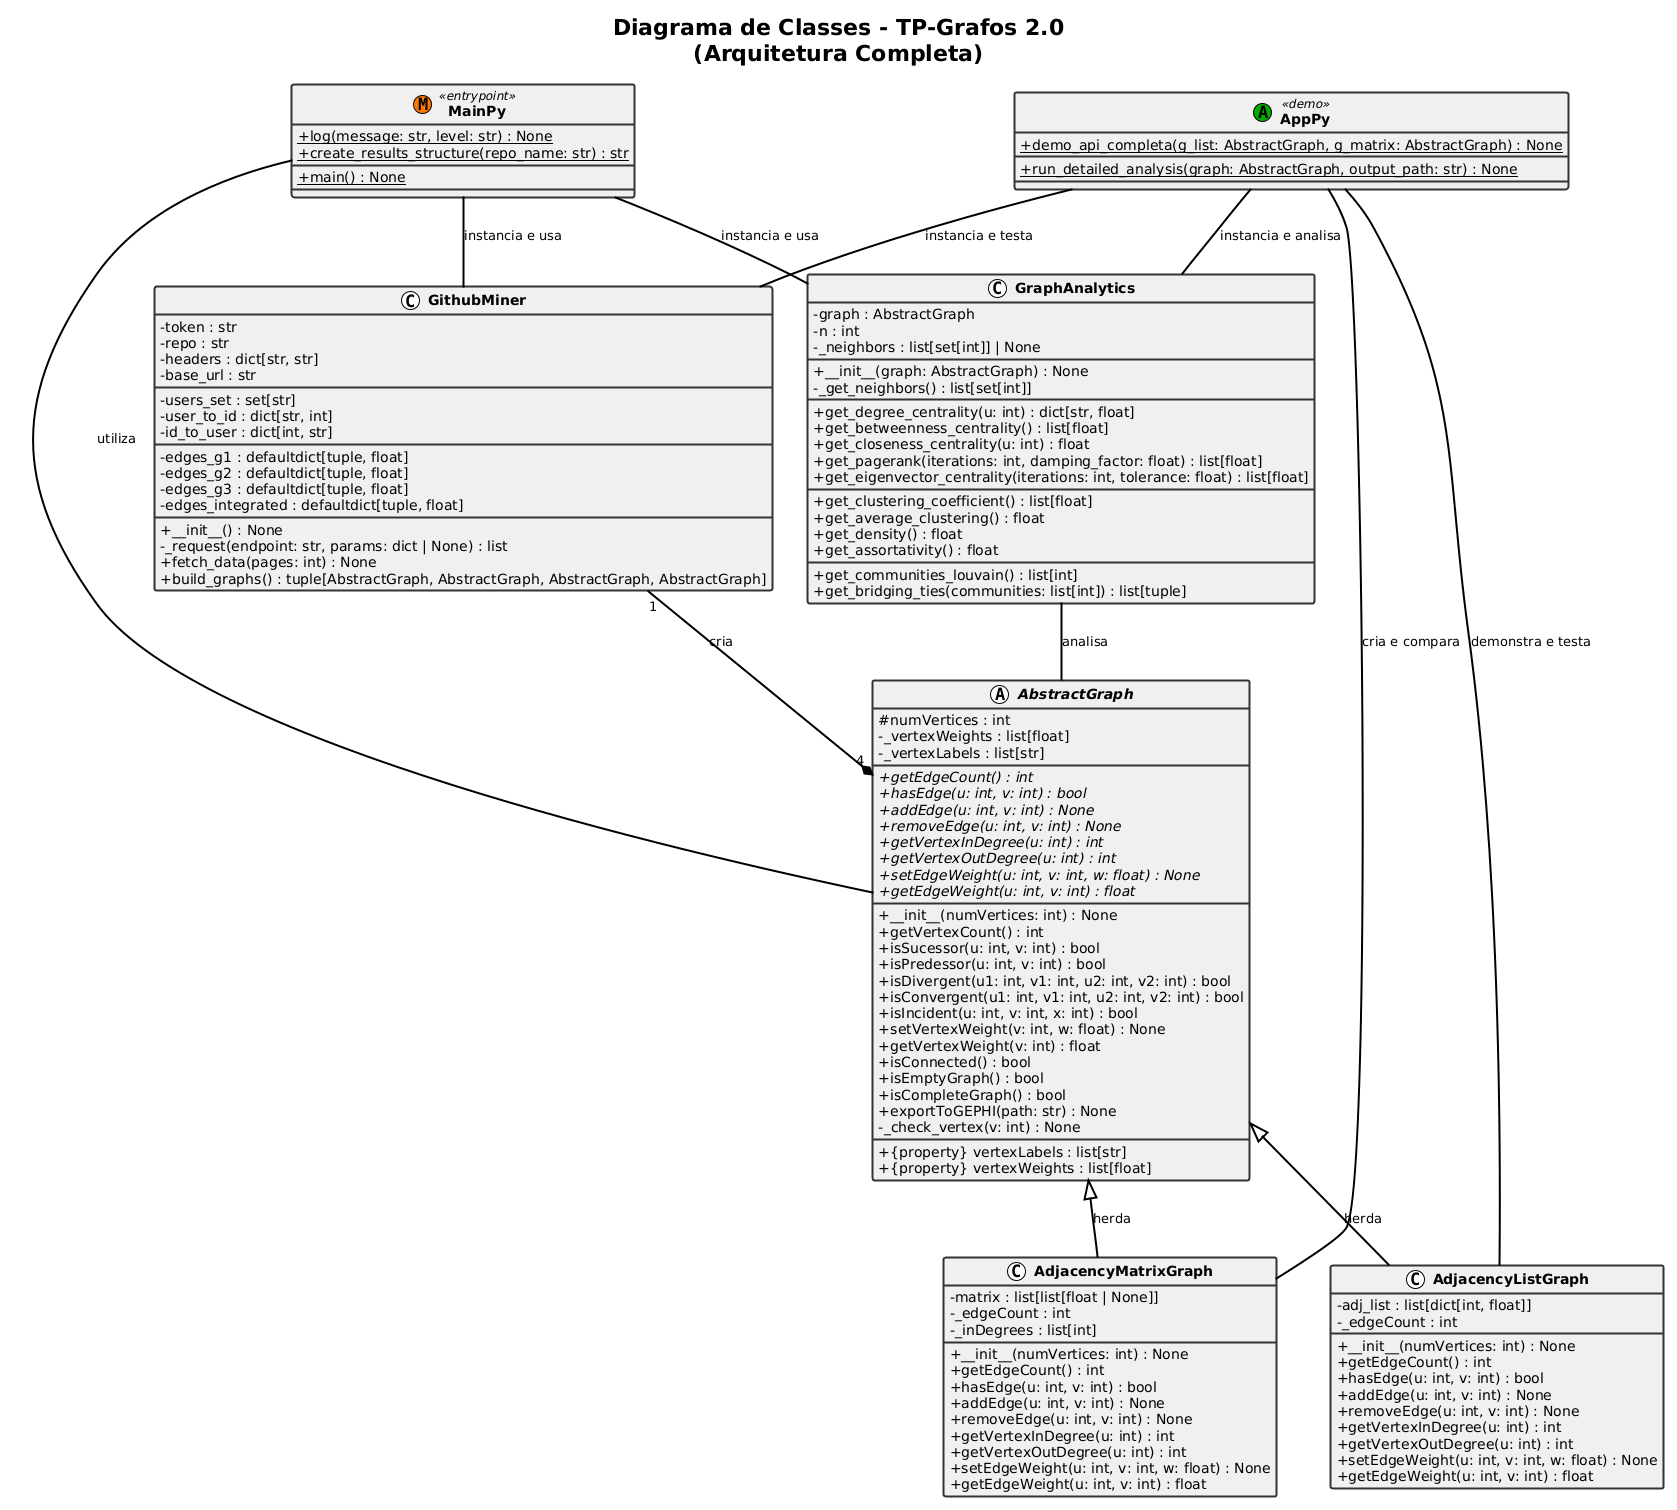
\includegraphics[width=\textwidth]{modelagem/Diagrama_de_classes.png}
    \caption{Estrutura de classes: AbstractGraph, implementações e módulos de mineração/análise.}
    \label{fig:diagrama-classes}
\end{figure}
% ----------------------------------------------------------------------------
\subsection{Diagrama de Componentes}
% ----------------------------------------------------------------------------

Arquitetura modular em cinco componentes: (i) \textit{Main Application} — orquestrador central; (ii) \textit{GitHub Miner} — coleta via API REST; (iii) \textit{Graph Storage} — instancia estruturas; (iv) \textit{Analytics Engine} — calcula métricas; (v) \textit{Export Module} — serializa em CSV e relatórios.

\begin{figure}[H]
    \centering
    
\includegraphics[width=\textwidth]{modelagem/diagrama_componentes.png}
    \caption{Arquitetura de componentes independentes.}
    \label{fig:diagrama-componentes}
\end{figure}

% ----------------------------------------------------------------------------
\subsection{Diagrama de Sequência — Mineração}
% ----------------------------------------------------------------------------

Narra a interação entre aplicação, minerador e API: (1) aplicação invoca \texttt{fetch\_data(pages=5)}; (2) minerador requisita \texttt{/repos/\{owner\}/\{repo\}/issues} com paginação; (3) para cada item: coleta comentários, revisões, merges; (4) respostas processadas, usuários agregados, pesos acumulados; (5) retorno com grafos instanciados.

\begin{figure}[H]
    \centering
    
\includegraphics[width=\textwidth]{modelagem/diagrama_sequencia_mineracao.png}
    \caption{Fluxo de interação durante coleta de dados.}
    \label{fig:diagrama-sequencia}
\end{figure}

% ----------------------------------------------------------------------------

% ============================================================================
% 4. ARQUITETURA DA FERRAMENTA
% ============================================================================
\section{Arquitetura da Ferramenta}\label{sec:arquitetura}

A ferramenta está organizada em 3 camadas:

\begin{figure}[h]
  \centering
  \begin{tikzpicture}[
    node distance=0.9cm,
    every node/.style={draw, rounded corners, minimum width=6cm, align=center, font=\small},
    app/.style={fill=yellow!20},
    analytics/.style={fill=orange!20},
    miner/.style={fill=blue!20},
    core/.style={fill=green!20},
  ]
    \node[app] (app) {\textbf{Aplicação}\\main.py, src/app.py};
    \node[analytics, below=of app] (analytics) {\textbf{Análise}\\GraphAnalytics};
    \node[miner, below=of analytics] (miner) {\textbf{Mineração}\\GithubMiner};
    \node[core, below=of miner] (core) {\textbf{Núcleo de Grafos}\\AbstractGraph, AdjacencyListGraph, AdjacencyMatrixGraph};

    \draw[-{Stealth[length=2mm]}, thick] (app) -- (analytics);
    \draw[-{Stealth[length=2mm]}, thick] (app) -- (miner);
    \draw[-{Stealth[length=2mm]}, thick] (miner) -- (core);
    \draw[-{Stealth[length=2mm]}, thick] (analytics) -- (core);
  \end{tikzpicture}
  \caption{Arquitetura em camadas da ferramenta.}
  \label{fig:arquitetura}
\end{figure}

\subsection{Camada 1: Núcleo de Grafos}

\texttt{AbstractGraph} define 20+ métodos: gerenciamento (getVertexCount, getEdgeCount), arestas (addEdge, removeEdge, hasEdge, pesos), graus (in/out-degree), relações (sucessor, predecessor, convergência), propriedades (conectividade, completude), exportação (exportToGEPHI em CSV).

\texttt{AdjacencyListGraph} usa listas de dicionários ($O(E)$ espaço, eficiente para redes esparsas). \texttt{AdjacencyMatrixGraph} usa matriz $N \times N$ (acesso $O(1)$ a arestas, cache de in-degrees).

\subsection{Camada 2: Mineração — \texttt{GithubMiner}}

Responsável por toda interação com a API REST do GitHub. Recebe token e repositório via \texttt{.env}.

\begin{itemize}
  \item \texttt{fetch\_data(pages)}: percorre issues e PRs, coleta comentários e revisões, acumula pesos em dicionários por tipo de grafo (\texttt{edges\_g1}, \texttt{edges\_g2}, \texttt{edges\_g3}, \texttt{edges\_integrated})
  \item \texttt{build\_graphs()}: mapeia logins para IDs sequenciais e instancia os 4 grafos como \texttt{AdjacencyListGraph}
\end{itemize}

\subsection{Camada 3: Análise — \texttt{GraphAnalytics}}

Recebe um \texttt{AbstractGraph} e implementa todos os algoritmos em Python puro, sem bibliotecas externas de grafos.

\subsection{Restrições Atendidas}

Sem bibliotecas externas (NetworkX); sem self-loops (verificação $u \neq v$); sem múltiplas arestas (acumulação de pesos); idempotência garantida; validação robusta de índices.

\subsection{Testes Unitários}

84 testes cobrindo: (i) API de grafos (ambas implementações): arestas, graus, relações, propriedades; (ii) mineração: mock da API, parsing, acumulação de pesos; (iii) casos extremos (grafos vazios, índices inválidos). Todos passam ✓.

\subsection{Aplicação de Demonstração}

\texttt{src/app.py} demonstra a API: criação de grafos, adição de arestas, consulta de graus, verificação de conectividade, exportação para Gephi.

% ============================================================================
% 5. MÉTRICAS E ANÁLISE
% ============================================================================
\section{Métricas e Análise}\label{sec:metricas}

Todas as métricas são implementadas na classe \texttt{GraphAnalytics} em Python puro.

\subsection{Centralidade de Grau}

\[
C_D(v) = \frac{\text{in-degree}(v) + \text{out-degree}(v)}{2(n-1)}
\]

In-degree = número de usuários que interagiram \textit{com} $v$; out-degree = número de usuários que $v$ interagiu \textit{com}.

\subsection{Betweenness Centrality}

\[
C_B(v) = \sum_{s \neq v \neq t} \frac{\sigma_{st}(v)}{\sigma_{st}}
\]

Onde $\sigma_{st}$ é o número de caminhos mais curtos entre $s$ e $t$, e $\sigma_{st}(v)$ é quantos passam por $v$. Implementado via algoritmo de Brandes $O(VE)$. Valor alto indica "conector" entre grupos.

\subsection{Closeness Centrality}

\[
C_C(v) = \frac{n-1}{\sum_{t \neq v} d(v,t)}
\]

Valor alto = colaborador próximo a todos (poucos hops).

\subsection{PageRank}

\[
\text{PR}(v) = \frac{1-d}{n} + d \sum_{u \to v} \frac{\text{PR}(u)}{\text{out-degree}(u)}
\]

Damping factor $d = 0{,}85$. Implementado via power iteration com convergência em $\epsilon = 10^{-6}$.

\subsection{Eigenvector Centrality}

\[
x_v = \lambda^{-1} \sum_{u \to v} x_u
\]

Resolvido via power iteration. Similar ao PageRank, mas sem damping factor.

\subsection{Clustering, Densidade, Assortatividade e Comunidades}

Clustering $C(v) = \frac{\text{arestas entre vizinhos}}{\binom{k_v}{2}}$ mede triângulos. Densidade $\rho = \frac{|E|}{|V|(|V|-1)}$ é proporção de conexões. Assortatividade (Pearson sobre graus) mede preferência de conexão. Louvain detecta comunidades. Bridging ties = usuários conectando múltiplas comunidades.

% ============================================================================
% 6. RESULTADOS E DISCUSSÃO
% ============================================================================
\section{Resultados e Discussão}\label{sec:resultados}

\subsection{Estatísticas Gerais}

A ferramenta foi executada sobre o repositório \texttt{devlikeapro/waha} (repositório de automação WhatsApp), coletando 5 páginas de issues e pull requests (máximo 500 itens). O dataset compreende o histórico completo de interações do repositório até a data de execução.

\begin{table}[h]
  \centering
  \caption{Estatísticas da rede analisada (repositório devlikeapro/waha).}
  \label{tab:stats}
  \begin{tabular}{l|r}
    \toprule
    \textbf{Métrica} & \textbf{Valor} \\
    \midrule
    Número de vértices (colaboradores únicos) & 481 \\
    Número de arestas — Grafo Integrado & 1409 \\
    Densidade da rede & 0,006103 \\
    Grafo fracamente conectado & Não \\
    Clustering médio & 0,148564 \\
    Assortatividade & $-0{,}249$ (dissortativo) \\
    Comunidades detectadas (Louvain) & 135 \\
    \bottomrule
  \end{tabular}
\end{table}

\subsection{Análise de Estrutura}

Densidade 0,006103: rede esparsa típica de open source. Clustering 0,1486: triângulos raros. Assortatividade $-0,249$: padrão dissortativo hub-and-spoke (hubs conectam-se com periféricos). 135 comunidades: reflete baixa coesão (muitos isolados de tamanho 1).

\subsection{Top 5 Colaboradores por PageRank e Centralidade}

\begin{table}[h]
  \centering
  \caption{Colaboradores mais influentes por PageRank (repositório devlikeapro/waha).}
  \label{tab:pagerank}
  \begin{tabular}{l|r|r}
    \toprule
    \textbf{Usuário} & \textbf{PageRank} & \textbf{In-Degree} \\
    \midrule
    devlikepro           & 0,11730 & 186 \\
    bergpinheiro         & 0,05065 & 86  \\
    vicentemarciot27     & 0,01745 & 22  \\
    OrionZap             & 0,01388 & 26  \\
    github-actions[bot]  & 0,01330 & 25  \\
    \bottomrule
  \end{tabular}
\end{table}

\textbf{Devlikepro:} PR 0,117 (8.8× top-2), in-degree 186, betweenness 0,619 (conecta 79/135 comunidades). Mantenedor principal. \textbf{Bergpinheiro:} PR 0,050, in-degree 86; co-mantenedor. \textbf{Padrão:} Top-5 concentram 21% do PageRank total (5/481 usuários).

\subsection{Exportação para Gephi}

CSV com colunas \texttt{Source}, \texttt{Target}, \texttt{Weight} (1409 arestas). Gephi: Import → Force Atlas 2 → Size by In-Degree → Color by Modularity. Visualiza núcleo central (top-5) e periferia esparsa.

% ============================================================================
% 7. RESPONSABILIDADES DOS INTEGRANTES
% ============================================================================


% ============================================================================
% 8. CONCLUSÃO
% ============================================================================
\section{Conclusão}\label{sec:conclusao}

Este trabalho implementou uma ferramenta completa de análise de redes de colaboração no GitHub:

\begin{enumerate}
  \item \textbf{Estruturas de dados:} \texttt{AbstractGraph} com duas implementações (\texttt{AdjacencyListGraph} e \texttt{AdjacencyMatrixGraph}), toda a API obrigatória implementada
  \item \textbf{Mineração:} \texttt{GithubMiner} com coleta de comentários, fechamentos, revisões e merges, construindo 4 grafos distintos
  \item \textbf{Métricas:} 10+ métricas em Python puro via \texttt{GraphAnalytics}
  \item \textbf{Exportação:} CSV compatível com Gephi via \texttt{exportToGEPHI}
  \item \textbf{Testes:} 84 testes unitários cobrindo a API de grafos e a mineração com mock
\end{enumerate}

============================================================================
% 9. REQUISITOS ATENDIDOS DO ENUNCIADO
% ============================================================================

\begin{thebibliography}{9}

\bibitem{brandes2001}
  Ulrik Brandes.
  \textit{A Faster Algorithm for Betweenness Centrality}.
  Journal of Mathematical Sociology, 25(2):163--177, 2001.

\bibitem{page1999}
  Lawrence Page, Sergey Brin, Rajeev Motwani, Terry Winograd.
  \textit{The PageRank Citation Ranking: Bringing Order to the Web}.
  Stanford InfoLab, 1999.

\bibitem{newman2010}
  M.\ E.\ J.\ Newman.
  \textit{Networks: An Introduction}.
  Oxford University Press, 2010.

\bibitem{gephi}
  Mathieu Bastian, Sebastien Heymann, Mathieu Jacomy.
  \textit{Gephi: an open source software for exploring and manipulating networks}.
  ICWSM, 2009.

\bibitem{github_api}
  GitHub Documentation.
  \textit{GitHub REST API}.
  https://docs.github.com/en/rest, 2024.

\end{thebibliography}

\end{document}
